\documentclass[10pt]{standalone}
\usepackage{pgfplots}
\pgfplotsset{compat=1.15}
\usepackage{mathrsfs}
\usetikzlibrary{arrows}
\pagestyle{empty}
\begin{document}
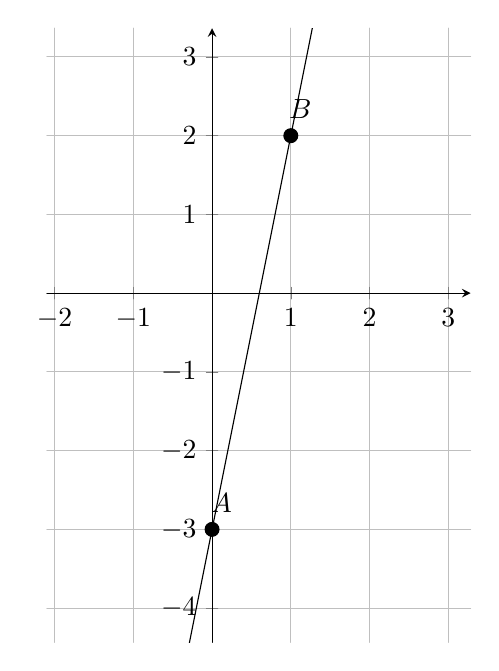
\begin{tikzpicture}[line cap=round,line join=round,>=triangle 45,x=1.0cm,y=1.0cm]
\begin{axis}[
x=1.0cm,y=1.0cm,
axis lines=middle,
ymajorgrids=true,
xmajorgrids=true,
xmin=-2.0981818181818244,
xmax=3.283636363636361,
ymin=-4.435418181818181,
ymax=3.3645818181818212,
xtick={-2.0,-1.0,...,3.0},
ytick={-4.0,-3.0,...,3.0},]
\clip(-2.0981818181818244,-4.435418181818181) rectangle (3.283636363636361,3.3645818181818212);
\draw [domain=-2.0981818181818244:3.283636363636361] plot(\x,{(--3.-5.*\x)/-1.});
\begin{scriptsize}
\draw [fill=black] (0.,-3.) circle (2.5pt);
\draw[color=black] (0.12,-2.662690909090908) node {$A$};
\draw [fill=black] (1.,2.) circle (2.5pt);
\draw[color=black] (1.12,2.337309090909094) node {$B$};
\end{scriptsize}
\end{axis}
\end{tikzpicture}
\end{document}